\section{Adaptations du jeu de données}

Une étape indispensable à la fouille de donnée réside dans le choix des attributs qui seront utilisés pour l'étude.
Il nous font donc y prêter une attention particulière, et choisir ceux qui nous paraissent les plus utiles, et essayer de réduire les dimensions et axes d'études.

\subsection{Corrélation d'attributs}

Afin de réduire les dimensions de l'étude, nous cherchons les corrélations entre les attributs disponibles. Voici les résultats pour le jeu \jeuc.

\begin{figure}[H]
	\begin{center}
		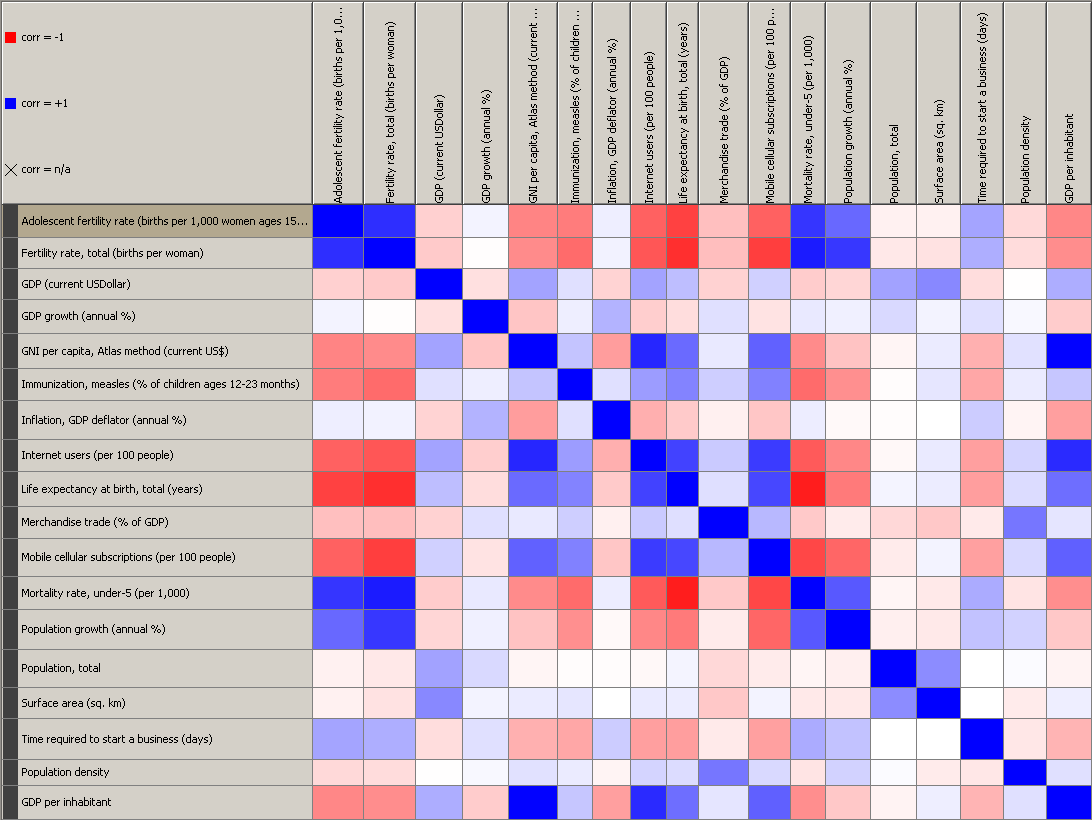
\includegraphics[scale=0.5]{Image/MatriceCorrelationNoMissing2}
		\caption{Matrice de corrélation pour le jeu \jeuc}
	\end{center}
\end{figure}

\subsection{Réduction des dimensions}

Au vu de ces résultat, nous estimons qu'une corrélation de 75\% minimum doublée d'une sémantique forte peut justifier la réduction de dimension. Nous utiliserons pour cela le compostant PCA.
 
Nous avons donc effectué les rapprochements suivants : 
\paragraph{Infrastructure} corrélation : 77\%
		\begin{itemize}
			\item Mobile cellular subscriptions
			\item Internet users
		\end{itemize}
\paragraph{TODODODODO} corrélation : 83\%
		\begin{itemize}
			\item Adolescent fertility rate
			\item Fertility rate
			\item Mortality rate ynder 5 years
		\end{itemize}
\hfill\\

De plus nous observons que certains attributs sont quelque peu redondants. Par exemple, GDP per Inhabitant (créé par nos soins) et GDI per capita sont corrélé à plus de 99\%. Nous n'utiliserons donc que ce second attribut, donné par \lesite .



